\section{Verification of Mobile Ad-hoc Protocols}\label{sec::wrebeca} 
Mobile Ad-hoc wireless networks (MANETs) consist of mobile nodes equipped by wireless transceivers by which they communicate. These networks are applicable where no pre-existing infrastructure, such as routers in wired networks or access points in managed (infrastructure) wireless networks are available, as their nodes operate in a completely collaborative and distributed manner. A node $A$ can receive data from a node $B$ if $A$ is located in the communication range of $B$, i.e., $A$ is directly connected to $B$. The union of (dis)connectivity relations among the node forms the underlying topology.  Due to the mobility of node, the (dis)connectivity relations may change, and the topology is dynamic. As all nodes are not directly connected, they rely on each other to communicate indirectly with those not within their range. To this aim, they collaborate ad-hocly to find a valid route to a destination. A route is valid if the corresponding path exists in the topology. Routes are partially maintained in the routing tables of nodes by indicating the next-hop(s) via which an intended destination is accessible. As topology changes, the routes maintained by nodes should be updated to prevent from useless communications leading to the energy consumption and network degradation. During the process of route maintenance, it is possible that by following next-hops, a route visits the same node more than once, and a loop is formed. To avoid data spinning over a MANET, \emph{loop-freedom} is one of the main properties of routing protocols MANET routing. Due to the enormous number of topology changes, finding a mobility scenario leading to protocol malfunction, e.g., the formation of a loop for routing protocols, is not possible by simulation-based approaches, and so these approaches can not assist in designing such protocols in practice. %without using rigorous analysis tools.   %designing MANET protocols is not easy in practice and  can be found by simulation-based approaches.  

%As wireless communication depends on the locality of nodes, i.e., the underlying topology, the behavior of nodes depends on the topology. Therefore, the correctness properties of MANETs are topology-dependent and hence, weaker in comparison with wired networks. For instance, one of the main properties of routing protocols is \emph{loop-freedom}, i.e., no established route stored in the routing tables visits the same node more than once. 
%\fixme{why "However"?}
%However, in MANETs, this property should hold for any mobility scenario. Another property for routing protocols is \emph{packet delivery}: always packets can be sent from a source to a connected destination. For MANETs, the packet delivery property is considered as whenever there is a path from a source to a destination for enough long period, any packet sent from a source can be received by the destination \cite{GlabbeekAWN}.

Rebeca is extended in \cite{FOAC}, called wRebeca, to model and verify %the topology-dependent properties of 
MANET protocols addressing dynamically changing topology. To support modeling such protocols, wRebeca provides unicast, multicast, and broadcast for communication. The wRebeca model of an abstract version of Ad-hoc On Demand Vector (AODV) routing protocol \cite{AODV} is given in Figure \ref{code:aodv}. Each node in the network is represented as an actor while the routing protocol
is modeled through the message servers of the actor. The network topology and its mobility are addressed by the state transition system, the third level of abstraction, and are not explicitly modeled in the wRebeca code.  
%
%\fixme{Long and confusing sentences (the ones below) - maybe you can use my friendliness paper for simpler explanation, I didn't check.}
In message server ${\it rec\_newpkt}$ (line $10$),
whenever a source node intends to send a data packet to a destination (${\it dip\_}$), %informed by receiving ${\it rec\_newpkt}$ from the upper-layer application, it will initiate the \emph{route discovery} procedure 
first it looks up in its routing table, ${\it rst}[{\it dip\_}]$, to see if it has a valid route to the destination to forward the data packet. Otherwise it starts a route discovery by broadcasting a route \emph{request} message, ${\it rec\_rreq}$, at line $16$. 
%
Nodes upon receiving a request message, forward the request if they do not have any route to the destination until the request reaches to the destination (line $24$). The destination replies by unicasting a \emph{reply} message, ${\it rec\_rrep}$, in response (line $26$) to the sender of the request (${\it oip\_}$). Due to unidirectional links, the sender may not be directly connected to the destination, so the destination unicasts to the next-hop toward the sender. The unicast message will be delivered
successfully ($\it succ$ in line $28$) if the receiver node is in the wireless range, or the
delivery can fail ($\it unsucc$ in line $31$) if the receiver node is not in the wireless range. The reply message is resent by the middle nodes until it arrives to the source node (line $48$).

\begin{figure*}
	\begin{center}
		%	\begin{lstlisting}[language=rebeca,multicols=2]
		\input{AODV.txt}
		%	\end{lstlisting}
	\end{center}
	\caption{The AODV protocol specified by wRebeca \label{code:aodv}\cite{FOAC}}
\end{figure*} 

To reason about small-sized networks by model checking technique, the state transition system of the model is generated. The global states %of a semantic model
are defined by the local state of rebecs and the underlying topology. The state-space generator produces two types of transitions; transitions for atomic handling of messages in actor queues, and transitions for random modification of the underlying topology to address mobility. For generating the first type, the effect of communication statements like broadcast is computed with respect to the topology. When an actor broadcasts, only those that are directly connected to the actor will receive the message. We remark that the underlying topology is not changed by the first type of transitions.   %As mobility is the intrinsic characteristic of nodes, the dynamism of the topology is not explicitly defined as part of the protocol specification. 
%To capture topology changes, for each global state, a set of state transitions are generated by which the underlying topology is randomly changed.  
For a network of $n$ nodes, there are $2\times \begin{pmatrix}
n \\
2 \\
\end{pmatrix}$ possible uni-directional links among them, and as each link can be up/down, there are $2^{(n^2-n)}$ possible topologies. %and by assuming the links are symmetrical, 
So, for each global state, $2^{(n^2-n)}$ transitions are generated to randomly change the topology, and the state pace grows exponentially. % in comparison with the classic Rebeca. 

\begin{figure}[h]
	\begin{subfigure}[b]{0.32\textwidth}
		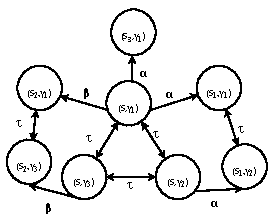
\includegraphics[width=\textwidth]{resources/st-before.pdf}
		\caption{Before reduction}\label{Fig::stbefore}	
	\end{subfigure}
	\begin{subfigure}[b]{0.14\textwidth}
		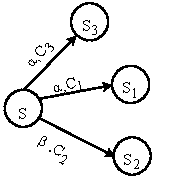
\includegraphics[width=\textwidth]{resources/st-after.pdf}
		\caption{After reduction}\label{Fig::stafter}	
	\end{subfigure}
	\caption{A simple state space before and after applying the reduction: $\tau$-transitions show the random changes of the topology while $\alpha/\beta-$transitions denote handling of message queues. The network constraint $C_1$ expresses the common links of the topologies $\gamma_{1}$ and $\gamma_2$ while $C_2$ represents the common links of $\gamma_1,\gamma_3$, and $C_3$ represents the links of $\gamma_1$.
	}\label{Fig::reductionidea}	
\end{figure}

To tackle the state-space explosion, we eliminate the topology from the global states and combine those states that are only different in their topologies. As a consequence, transitions modifying the topology are removed (as they become self-loop $\tau$-transitions). So states $(S,\gamma_1)$, $(S,\gamma_2)$, and $(S,\gamma_3)$, where $S$ and $\gamma_i$ denote the local states of rebecs and topology respectively, are aggregated as demonstrated in Figure \ref{Fig::stafter}. %A transition is defined from $S$ to $S_1$ if there exists $\gamma_1$ such that $(S,\gamma_1)\overto (S_1,\gamma_1)$. 
To capture the effect of topology on the state transitions of the reduced model, the (dis)connectivity of those links that results the same modification on the local states of actors %in the original model 
are added to the labels on the transitions. For example, $S\overto{\alpha} S_1$ is possible in Figure \ref{Fig::stafter} when the underlying topology is either $\gamma_1$ or $\gamma_2$. The links common in both $\gamma_{1}$ and $\gamma_{2}$ that result in the same local state modification, i.e., $S_1$ in Figure \ref{Fig::stbefore}, are added to the label of the transition in Figure \ref{Fig::stbefore}. It should be noted that due to non-determinism in the wRebeca model, $(S,\gamma_1)\overto{\alpha}(S_3,\gamma_1)$, leading to a non-determinism in the reduced model. A set of (dis-)connectivity relations among two actors, expressing the status of their links, is called \emph{network constraint}~\cite{FatemehFI10,FatemehFI19}. For instance, ${\it and}({\it con}(n_1,n_2),!{\it con}(n_3,n_4)$ denotes that the actor  $n_1$ is connected to $n_2$ while $n_3$ is disconnected from $n_4$. The network constraints on transitions express the conditions that the combined states have symmetric behaviors. Our reduction technique is indeed a form of symmetric reduction technique \cite{clarke1998symmetry}. This form of reduction can be applied if the actors were not isolated. %; it is independent from the  
However, the isolation of actors makes this reduction more effective for the analysis of real-world protocols like AODV.  
%TODO::why this is possible
%The network constraint of each state transition isolates those connected actors and computes the effect of processing of events. 



%an event while isolating those connected actors. %while it is restricted to the set of topologies for which that behavior is valid. 

We elaborate the idea with a concrete example on AODV. Consider a MANET with four nodes $n_1$, $n_2$, $n_3$, and $n_4$, where $n_1$ and $n_3$ are the source and destination, respectively, and $n_3$ has a request message to handle, received from $n_2$. Recall that a destination node, upon receiving a request message, ${\it rec\_rreq}$, unicasts ${\it rec\_rrep}$ to the next-hop of the request origin $({\it oip\_})$ (line $26$ in Figure \ref{code:aodv}). We consider that the next-hop for $n_3$ to reach $n_2$ is through $n_4$. The state in which $n_3$ has a route request message to handle is determined with a thick border in Figure \ref{Fig::reduction}. As a consequence of handling the route request, two categories of state-transitions are generated; one for the case that the destination $n_3$ is connected to $n_4$, denoted by $\{n_3\nconn n_4\}$, and one for the case that it is disconnected, denoted by $\{n_3\nconn n_4\}$. In the first case, %the destination and next-hop are considered in isolation and 
the effect of processing a route request message is computed by inserting a ${\it rec\_rrep}$ message in the queue of $n_4$. In the second case, $n_3$ will inform its upstream nodes that $n_4$ is not reachable through it anymore by broadcasting an error message, ${\it rec\_rerr}$ (this part of code has been abstracted in line $33$). %So, the state-transitions are partitioned in further to %In other words, the effect of processing the request event is computed for those connected subsets of actors excluding the next-hop in isolation. 
%The state space of this scenario has been illustrated in Figure \ref{Fig::reduction}. % Assume that $n_1$ and $n_3$ are the source and destination, respectively, and $n_3$ has received its request message from $n_2$. The next-hop for $n_3$ to reach $n_2$ is through $n_4$. The state in which $n_3$ has a request message to handle is determined with a thick border. The next states are classified into two categorizes; those that $n_3$ is connected to $n_4$, denoted by $\{n_3\conn n_4\}$, and those that $n_3$ is disconnected from $n_4$, denoted by $\{n_3\nconn n_4\}$. 
Thus the second category is partitioned regarding the connectivity of $n_3$ to $n_1$ and $n_2$. When $\{n_3\nconn n_1,n_2,n_4\}$, %the next state is computed for $n_3$ in isolation with no neighbour to receive the error message, so 
none of the nodes $n_1$ and $n_2$ are affected. Conversely when $\{n_3\nconn n_4\},\{n_4\conn n_1,n_2\}$, %the next state is computed for $n_1,n_2,n_3$ in isolation, so 
both $n_1$ and $n_2$ get the error message. To enforce a set of stable (dis)connectivity relations among the actors to govern the level of partitioning, they can be specified in \emph{constraints} block at line $68$ of Figure \ref{code:aodv}. For instance, this given network transition enforces $n_3\conn n_4$, so only the first category of state-transitions is possible in Figure \ref{Fig::reduction}. 
\begin{figure}
	%\begin{tikzpicture}[scale=.8, transform shape]
	%	\input{reductionFig.tex}
	%\end{tikzpicture}
	%---------------------
	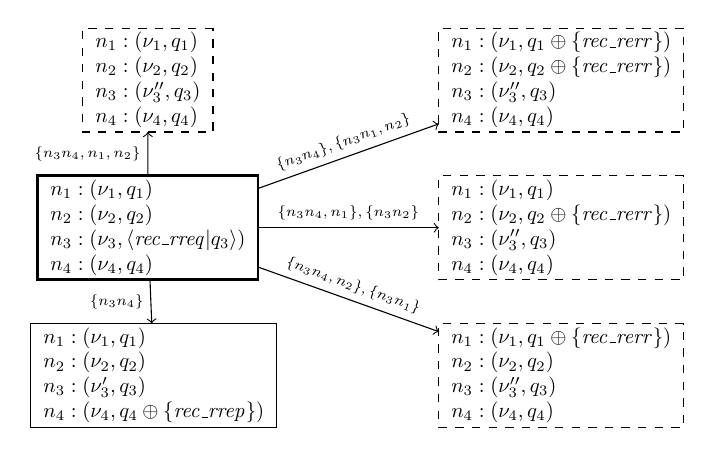
\begin{tikzpicture}[scale=.75, transform shape]
	\node [draw,outer sep=0,inner sep=1,minimum size=10,line width=1pt] (n1) at (0,-0.5) {$\begin{array}{l} 
		n_1:(\nu_1,q_1)\\ 
		n_2:(\nu_2,q_2)\\
		n_3:(\nu_3,\langle {\it rec\_rreq}|q_3\rangle)\\
		n_4: (\nu_4,q_4)
		\end{array}	$};
	\node [draw,outer sep=0,inner sep=1,minimum size=10] (n2) at (0.1,-3)
	{$\begin{array}{l} 
		n_1:(\nu_1,q_1)\\ 
		n_2:(\nu_2,q_2)\\
		n_3:(\nu_3',q_3)\\
		n_4:(\nu_4,q_4\oplus \{{\it rec\_rrep}\})\\
		\end{array}$};
	\node [draw,outer sep=0,inner sep=1,minimum size=10, style=dashed] (n3) at (7,2)
	{$\begin{array}{l} 
		n_1:(\nu_1,q_1\oplus \{{\it rec\_rerr}\})\\ 
		n_2:(\nu_2,q_2\oplus \{{\it rec\_rerr}\})\\
		n_3:(\nu_3'',q_3)\\
		n_4:(\nu_4,q_4)\\
		\end{array}$};
	\node [draw,outer sep=0,inner sep=1,minimum size=10, style=dashed] (n4) at (7,-0.5)
	{$\begin{array}{l} 
		n_1:(\nu_1,q_1)\\ 
		n_2:(\nu_2,q_2\oplus \{{\it rec\_rerr}\})\\
		n_3:(\nu_3'',q_3)\\
		n_4:(\nu_4,q_4)\\
		\end{array}$};
	\node [draw,outer sep=0,inner sep=1,minimum size=10, style=dashed] (n5) at (7,-3)
	{$\begin{array}{l} 
		n_1:(\nu_1,q_1\oplus \{{\it rec\_rerr}\})\\ 
		n_2:(\nu_2,q_2)\\
		n_3:(\nu_3'',q_3)\\
		n_4:(\nu_4,q_4)\\
		\end{array}$};
	\node [draw,outer sep=0,inner sep=1,minimum size=10, style=dashed] (n6) at (0,2)
	{$\begin{array}{l} 
		n_1:(\nu_1,q_1)\\ 
		n_2:(\nu_2,q_2)\\
		n_3:(\nu_3'',q_3)\\
		n_4:(\nu_4,q_4)\\
		\end{array}$};
	\draw[->] (n1) edge node[left]{\scriptsize$\{n_3\conn n_4\}$} (n2);
	\draw[->] (n1) edge[sloped,above] node{\scriptsize $\{n_3\nconn n_4\},\{n_3\conn n_1,n_2\}$} (n3);
	\draw[->] (n1) edge node[above]{\scriptsize$\{n_3\nconn n_4,n_1\}, \{n_3\conn n_2\}$} (n4);
	\draw[->] (n1) edge[sloped,above] node{\scriptsize$\{n_3\nconn n_4,n_2\},\{n_3\conn n_1\}$} (n5);
	\draw[->] (n1) edge node[left]{\scriptsize$\{n_3\nconn n_4,n_1,n_2\}$} (n6);
	\end{tikzpicture}   	
	\caption{Possible next states upon handling of a request message: connectivity and disconnectivity relations are represented by the notation $\conn $ and $\nconn$, respectively. The next states are classified into two categorizes; those as a consequence of $\{n_3\conn n_4\}$ are shown with solid border, while those as a consequence of $\{n_3\nconn n_4\}$ are shown with dashed border. The notation $\langle m|q\rangle$ expresses a queue with head $m$ and tail $q$ and $q\oplus\{m\}$ shows the queue $q$ that the item $m$ has been appended to its end.}\label{Fig::reduction}
\end{figure}
%
This reduction approach shrinks the state space substantially for real-world protocols and hence, makes the model checking technique possible as shown in Table \ref{Tab:aodv-redu}. When the number of nodes increases from $4$ to $5$ for AODV while the network constraint results only $16$ possible topologies, the classic state space cannot be generated due to the memory limitation on a computer with $8${GB} {RAM}.  We proved that the reduced state space is branching bisimilar to the
original one, and consequently a set of properties such as {ACTL-X} are preserved \cite{FOAC}. The network constraints on transition are used during model checking \cite{FORM,CSI2018} to verify the topology-sensitive properties. 

\begin{table*}
	%   \renewcommand{\arraystretch}{1.5}
	\centering
	\caption{Comparing the size of state spaces with/without applying reduction \cite{FOAC}}
	\begin{tabular*}{0.75\textwidth}{@{\extracolsep{\fill }} |   c  c  r  r  r  r  |   }
		\hline
		No. of & No. of valid & No. of states    &  No. of transitions     & No. of states & No. of transitions
		\\
		nodes & topologies & before reduction  &  before reduction   & after reduction &  after reduction
		\\
		\hline	     
		4 & 4 & 3,007 & 16,380 & 763  & 1,969 \\
		4  & 8 & 12,327 & 113,480 & 1,554  & 3,804 \\
		4  & 16 & 35,695 & 610,816 & 2,245 & 5,549 \\    
		4  & 32 & 93,679 & 3,097,792 & 2,942 & 7,596 \\  
		4    & 64  & 258,447  & 16,797,536 & 4,053 & 10,629 \\
		5 & 16 & $>$655,441 & $>$11,276,879 & 165,959 &  598,342 \\
		\hline
	\end{tabular*}
	\label{Tab:aodv-redu}
\end{table*}

The reduction technique can be improved further if the topology be stable %. As rebecs have no shared variable, the state space %of a network, consisted of homogeneous nodes, 
%can be reduced 
by applying \emph{counter abstraction} technique \cite{emerson1999asymmetry}. This technique is also considered of symmetric reduction. By this technique, the global state is recorded by a vector of counters, one for each local state of nodes. If there are $n$ nodes in a network where each node can have $m$ possible local states, the global state is shown as $\langle c_1,\ldots,c_m \rangle $, where $c_i\le n$ denotes the number of nodes residing in the local state $i\le m$. Therefore, the state space is reduced from $m^n$ to $\begin{pmatrix}
n+m-1 \\
m \\
\end{pmatrix}$. To apply
counter abstraction concerning the topology, rebecs with an identical local state and
neighbors, called \textit{topologically equivalent},  are counted together. Intuitively, all topologically equivalent nodes should be either all connected to each other, or disconnected, while they should have the same neighbors (except themselves). So if either one broadcasts, the same set of nodes (except themselves) will receive, and if they are also connected to each other, their counterpart (that is symmetric to the sender) will receive. For example, the nodes $1,3$ and $2,4$ are topologically equivalent in Figure \ref{fig:topequiv}. To compute the reduced state space, nodes of the underlying topology are partitioned into the maximal sets of topologically equivalent nodes, and then a counter is considered for each pair of topology equivalence class and a local state that a rebec can reside in. For instance, assume a network with four rebecs of the same class where $i$ and ${\it msg}$ are its state variable and message server name, respectively. When the underlying topology is the one shown in Figure \ref{fig:topequiv}, as rebecs $1$ and $3$ have the same local state (expressed by a pair of the state variable valuation and message queue) as shown in Figure \ref{fig::reduction}, and they are topologically equivalent, the global state can be represented as shown in this figure. As a consequence, the resulting state merges two states into one: one as shown in the figure, and the other in which the local states of nodes $2$ and $4$ swap. We proved that the reduced transition system is strongly bisimilar to
the original one, and the state space reduction is considerable for models with homogeneous  actors that are no more distinguished by their identifiers. This technique is
beneficial for finding an error when modifying a protocol. If we found an error for a certain topology, %leads to an error %malfunctioning of a previous version of the protocol, 
we can check the new version of the protocol using that certain topology.

\begin{figure*}
	\centering
	\begin{subfigure}[b]{0.3\textwidth}
		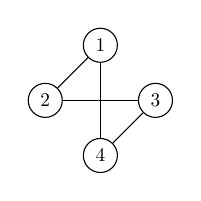
\begin{tikzpicture}[scale=.7, transform shape]
		\node[style=circle,draw] (n1) at (1,2) {$1$};
		\node[style=circle,draw] (n2) at (0,1) {$2$};
		\node[style=circle,draw] (n3) at (2,1) {$3$};
		\node[style=circle,draw] (n4) at (1,0) {$4$};
		\draw (n1) edge (n2);
		\draw (n1) edge (n4);
		\draw (n3) edge (n2);
		\draw (n3) edge (n4);
		\end{tikzpicture}
		\caption{A topology: the links among the nodes are bidirectional}
		\label{fig:topequiv} 	
	\end{subfigure}
	\begin{subfigure}[b]{0.6\textwidth}
		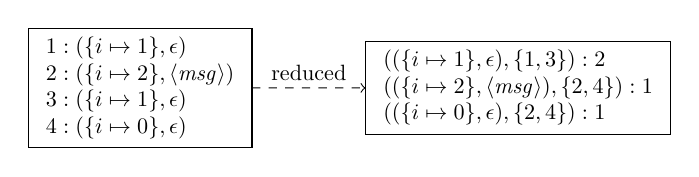
\begin{tikzpicture}[scale=.8, transform shape]
		\node [draw,outer sep=0,inner sep=3,minimum size=10] (n1) at (1,11) {$\begin{array}{l} 
			1:(\{i\mapsto 1\},\epsilon)\\ 
			2:(\{i\mapsto 2\},\langle{\it msg}\rangle)\\
			3:(\{i\mapsto 1\},\epsilon)\\
			4:(\{i\mapsto 0\},\epsilon)\end{array} %\begin{pmatrix}
			$};
		\node [draw,outer sep=0,inner sep=3,minimum size=10] (n2) at (7,11)
		{$\begin{array}{l} ((\{i\mapsto 1\},\epsilon),\{1,3\}):2
			\\((\{i\mapsto 2\},\langle{\it msg}\rangle),\{2,4\}):1\\
			((\{i\mapsto 0\},\epsilon),\{2,4\}):1\end{array} $};
		\draw[->, style=dashed] (n1) edge node[above]{reduced} (n2);
		\end{tikzpicture}
		\caption{Counter abstraction reduction}
		\label{fig::reduction}
	\end{subfigure}    	
	\caption{Applying counter abstraction reduction to a network with four nodes and the assumed topology, each having a local variable $i$ }
	\label{fig:counter-abstraction}
\end{figure*}


%To characterize the timing-dependent behavior of such protocols concerning mobility scenarios, Timed Rebeca was extended orthogonally with the topology concepts of wRebeca. For instance, the mobility scenario over which the maximal response time to find a routing path can be extracted via model checking technique. This was achieved by combining the floating-time idea of Timed Rebeca with network constraints exploited in wRebeca. 